\documentclass[12pt,aspectratio=169]{beamer}

\usetheme[progressbar=frametitle]{metropolis}
% \usetheme[outer/progressbar=foot]{metropolis}
% \usetheme[outer/progressbar=foot,outer/numbering=none]{metropolis}

% \setsansfont[BoldFont={Source Sans Pro Semibold},
%               Numbers={OldStyle}]{Source Sans Pro}

% \setsansfont{Lato}
% \usepackage{eulervm}

\usepackage{appendixnumberbeamer}
% \metroset{titleformat=smallcaps}
\usepackage{booktabs}
\usepackage[scale=2]{ccicons}

\usepackage{pgfplots}
\usepgfplotslibrary{dateplot}
\usepackage{hyperref}
\usepackage{graphicx}
\usepackage[justification=centering,skip=0pt]{caption}
\usepackage{amssymb,amsmath,amsthm} 
\usepackage{colortbl}
\usepackage{pdflscape}
\usepackage{xpatch, animate}
\usepackage[super]{nth}
\usepackage{threeparttable}
\usepackage{makecell}
\usepackage{subcaption}
\usepackage{bm}
\usepackage{nth}
\usepackage{multimedia}

\usepackage{xspace}
\newcommand{\themename}{\textbf{\textsc{metropolis}}\xspace}
\newenvironment{wideitemize}{\itemize\addtolength{\itemsep}{10pt}}{\enditemize}
\providecommand{\propositionname}{Proposition}
\setbeamertemplate{frametitle continuation}[from second][(contd.)]

\newcommand{\vspM}{\vspace{0.12truecm}}
\newcommand{\vspI}{\vspace{0.75truecm}}
\newcommand{\vspH}{\vspace{0.45truecm}}
\newcommand{\vspII}{\vspace{1.8truecm}}
\newcommand{\hspI}{\hspace{1truecm}}
\newcommand{\hspII}{\hspace{1.8truecm}}
\newcommand{\hspIV}{\hspace{3.8truecm}}

\definecolor{yellow}{RGB}{240,228,66}
\definecolor{green}{RGB}{0,158,115}
\definecolor{blue}{RGB}{0,114,178}
\definecolor{red}{rgb}{0.85,0.325,0.098}%{RGB}{213,94,0}
\definecolor{yellow}{RGB}{240,228,66}
\definecolor{green}{RGB}{0,158,115}
\newenvironment{transitionframe}{
	\setbeamercolor{background canvas}{bg=mDarkBrown}
	\begin{frame}[plain, noframenumbering]}{
	\end{frame}
}
\setbeamercolor{block body}{bg=mDarkTeal!20}
\setbeamercolor{block title}{bg=mDarkTeal!90,fg=black!2}
\usetikzlibrary{arrows,positioning} 
\tikzset{hl/.style={
		set fill color=red!80!black!40,
		set border color=red!80!black,
	},
}

\newtheorem{prop}{\protect\propositionname}
\providecommand{\propositionname}{Proposition}

\definecolor{Purple}{HTML}{911146}
\definecolor{Orange}{HTML}{CF4A30}

% % Theme colors are derived from these two elements
% \setbeamercolor{alerted text}{fg=Orange}

% % ... however you can of course override styles of all elements
% \setbeamercolor{frametitle}{bg=Purple}

% \metroset{titleformat=smallcaps}
%%%%%%%%%%%%%%%%%%%%%%%%%%%%%%%%%%%%%%%%%%%%%
% \documentclass[12pt, aspectratio=169]{beamer}
% \usepackage{amsmath, amsfonts, amssymb, amsthm,pstricks,psfrag,pst-node,pst-text,pst-3d,pgf,soul, graphics}
% \setbeamertemplate{footline}[frame number]

% \usepackage[T1]{fontenc}
% \usepackage{helvet}
% \usepackage[default]{lato}
% \usepackage{array}

% %\definecolor{blue}{RGB}{0,114,178}
% \definecolor{blue}{rgb}{0,0.28,0.67}
% \definecolor{red}{RGB}{213,94,0}
% \definecolor{yellow}{RGB}{240,228,66}
% \definecolor{green}{RGB}{0,158,115}

% %% I use a beige off white for my background
% \definecolor{MyBackground}{RGB}{255,253,218}

% %\usetheme[progressbar=frametitle]{metropolis}
% \setbeamertemplate{frametitle continuation}[from second][(contd.)]
% \newenvironment{wideitemize}{\itemize\addtolength{\itemsep}{10pt}}{\enditemize}
% \setbeamertemplate{navigation symbols}{}
% \setbeamertemplate{theorems}[numbered]

% \setbeamercolor{frametitle}{fg=blue}
% \setbeamercolor{title}{fg=black}
% \setbeamertemplate{footline}[frame number]
% \setbeamertemplate{navigation symbols}{} 
% %\setbeamertemplate{itemize items}{-}
% \setbeamertemplate{itemize items}[circle]
% \setbeamercolor{itemize item}{fg=blue}
% \setbeamercolor{itemize subitem}{fg=blue}
% \setbeamercolor{enumerate item}{fg=blue}
% \setbeamercolor{enumerate subitem}{fg=blue}
% \setbeamercolor{button}{bg=MyBackground,fg=blue,}

% \newcommand{\vspM}{\vspace{0.12truecm}}
% \newcommand{\vspI}{\vspace{0.75truecm}}
% \newcommand{\vspH}{\vspace{0.45truecm}}
% \newcommand{\vspII}{\vspace{1.8truecm}}
% \newcommand{\hspI}{\hspace{1truecm}}
% \newcommand{\hspII}{\hspace{1.8truecm}}
% \newcommand{\hspIV}{\hspace{3.8truecm}}

% \newcommand{\E}{\mathbb{E}}
% \newcommand{\var}{\mathrm{Var}}
% \newcommand{\cov}{\mathrm{Cov}}

% \newenvironment{transitionframe}{
%   \setbeamercolor{background canvas}{bg=black}
%   \begin{frame}}{
%     \end{frame}
% }

% \newtheorem{prop}{\protect\propositionname}
% \providecommand{\propositionname}{Proposition}
% \usepgfplotslibrary{external}
% \tikzexternalize
\title{Dissecting the Aggregate Market Elasticity}
\date{\today}
\author[Short Name (U ABC)]{%
	\texorpdfstring{%
		\begin{columns}
			\column{.25\linewidth}
			\centering
			Victor Duarte \\ {\small UIUC}
			\column{.25\linewidth}
			\centering
			Mahyar Kargar \\ {\small UIUC}
			\column{.25\linewidth}
			\centering
			Dejanir Silva \\ {\small Purdue}			
		\end{columns}		
		\vspace{15pt}
		\begin{columns}
			\column{\linewidth}		
		\end{columns}
	}
	{Author 1, Author 2, Author 3}
}


\begin{document}

\maketitle

\begin{frame}{Why is the aggregate stock market so price-inelastic?}
    \begin{wideitemize}
        % \item Large stock price movements in response to small flows\vspM
        \item Stock prices are very sensitive to flows\vspM
        \begin{itemize}
            %\item what happens when one sells \$1 in bonds and buys \$1 of stocks?
            \item if there is a 1\% flow {\scriptsize(as a frac. of equity values)} from bonds to stocks
            %\item the aggregate stock market goes up by \$5
            \item the equity market value goes up by 5\%
            \item \textbf{inelastic market hypothesis} {\scriptsize(Gabaix-Koijen, 2020)}
        \end{itemize}
        \item Can frictionless models generate a low aggregate elasticity?
        \item If not, what frictions help explain large price movements?
        \item Understanding this helps us answer a key open puzzle:\vspM
        \begin{itemize}\normalsize
            \item the origins of \textbf{high stock market volatility}
        \end{itemize}
        
    \end{wideitemize}
\end{frame}

\begin{frame}{This paper}
    \begin{wideitemize}
        \item Provide a framework to answer these questions
        \item Quantitative GE model with rich investor heterog. \& financial frictions
        \item The \textbf{general equilibrium} perspective is key for \textbf{macro} elasticity
        \begin{itemize}
            \item most existing work is PE and/or with limited/no heterogeneity
        \end{itemize}
        \item Using perturbation methods to obtain analytical solution
        \item We consider two types of frictions
        \begin{itemize}
            \item passive investments by households
            \item heterog. active investors who face leverage constraints
        \end{itemize}
    \end{wideitemize}
\end{frame}

\begin{frame}{Results (so far)}
   \begin{wideitemize}
       \item Volatility depends on \textbf{aggregate elasticity} and \textbf{flow shocks}
       \item Aggregate elasticity:
       \begin{itemize}
           \item is state-dependent: wealth distribution matters
           \item no price impact of flows in frictionless settings (infinite elasticity)
           \item adding passive investors makes market more inelastic
           \item preference heterog. attenuates the price impact (risk misallocation)
           \item binding leverage constraints amplifies the price impact
       \end{itemize}
       \item Decompose the price impact into components due to:
       \begin{itemize}
           \item risk premium
           \item risk-free rate
           \item price drift
       \end{itemize}
   \end{wideitemize} 
\end{frame}

\begin{frame}{Literature}
    \begin{wideitemize}
        \item \textcolor{blue}{Aggregate (macro)} demand elasticity:\\ {\footnotesize ``change in agg. stock market's value in response to a \$1 flow to stocks from bonds''}
        \begin{itemize}
            \item {\scriptsize Johnson (2006), Deuskar-Johnson (2011), Gabaix-Koijen (2021), Haddad-Huebner-Loualiche (2021), Li-Pearson-Zhang (2021)}
        \end{itemize}
        \item \textcolor{red}{Micro} demand elasticity:\\
        {\footnotesize ``change in relative price of stocks $A$ and $B$ if one buys \$1 of $A$, and sells \$1 of $B$''}
        \begin{itemize}
            \item {\scriptsize Shleifer (1986), Wurgler-Zhuravskaya (2002), Chang-Hong-Liskovich (2014), Koijen-Yogo (2019)}
            \item higher elasticity than the aggregate market 
        \end{itemize}
        \item Heterogeneous agent models with financial frictions
        \begin{itemize}
            \item {\scriptsize Basak-Cuoco (1998), Gârleanu-Pedersen (2011), Longstaff-Wang (2012), Gârleanu-Panageas (2015), Silva (2020), Kargar (2021)}
        \end{itemize}
    \end{wideitemize}
\end{frame}

\begin{frame}[standout]
        Model
\end{frame}

% \begin{transitionframe}
%   \begin{center}
%     { \Huge \textcolor{black}{Model}}
%   \end{center}
% \end{transitionframe}

\begin{frame}{Assets and endowments}
    \textcolor{blue}{Endowment:} continuous time, infinite horizon, endowment economy 
    \[\frac{d Y_{t}}{Y_{t}}=\mu dt+\sigma dZ_{t}%\pause
    \]
    
    \vspM
    \textcolor{blue}{Markets:} agents have access to two assets
    \begin{itemize}
        \item a riskless asset in zero net supply
        \item a risky claim on the aggregate endowment in unit supply
    \end{itemize}
    \vspM
    \textcolor{blue}{Asset return:}
    \[ d R_t = \frac{d P_t + Y_t dt}{P_t} \equiv \mu_{R,t} dt + \sigma_{R,t}\, d Z_t,\]
    \begin{itemize}
        \item $\mu_R$ and $\sigma_R$ determined in equilibrium
    \end{itemize}
    % \textcolor{blue}{Agents:} Economy populated by \textbf{passive} and \textbf{active} investors
    % \begin{itemize}
    % 	\item Unit measure of investors facing frictions in the risky asset market \vspM
    % 	\item Unit measure of risk-neutral dealers who hold no inventory
    % \end{itemize}
\end{frame}

\begin{frame}{Investors}
\begin{wideitemize}
    \item $J+1$ types: $j=0,1,\ldots, J$ with mass $\omega_j$
    \item Agents die at rate $\kappa$; mass $\kappa\omega_j$ born every period {\scriptsize (to make the model stationary)}
    \item All agents have Duffie-Epstein recursive preferences\vspM
    \begin{itemize}\normalsize
        \item risk aversions $\gamma_j$ and common EIS $\psi$
    \end{itemize}
    \item Choose consumption $C_{j,t}$ and portfolio weight in risky asset $\alpha_{j,t}$
    \item Two investor categories: Active \& Passive
\end{wideitemize}
\end{frame}

\begin{frame}{Investors (contd.)}
\begin{wideitemize}
    \item \textcolor{blue}{Passive investors:}
    \begin{itemize}
        \item  type $j=0$; have portfolio share $\alpha_{0,t}=\overline{\alpha}_{p,t}$ follow an exog. CIR process:
        \[d \overline{\alpha}_{p, t}=\theta_{p}\left(\overline{\alpha}-\overline{\alpha}_{p, t}\right) d t+\sigma_{p} \sqrt{\overline{\alpha}_{p, t}}\, d Z_{t}\]
        \item captures fluctuations in the passive investors risky asset holding\vspM
        \item innovations to $\overline{\alpha}_p$: \textbf{portfolio flow shocks}\vspM
        \item movements in $\overline{\alpha}_p$: due to agg. and/or indep. pure flow shocks\vspM
        %\textcolor{red}{say something about bivariate $dZ$ pure flow shocks/correlated with aggregate}
    \end{itemize}
    \item \textcolor{blue}{Active investors:} 
    \begin{itemize}
        \item type $j=1,\ldots,J$; continuously rebalance their portfolios\vspM
        \item face state-dependent \textbf{leverage constraints}
        \[\alpha_{j, t} \leq \frac{\overline{\sigma}}{\left\|\sigma_{R, t}\right\|}\]
    \end{itemize}
\end{wideitemize}
\end{frame}

\begin{frame}{Investors' problem}
Investor type $j$'s problem
    \[V_{j, t}=\max _{\left\lbrace C_{j}, \alpha_{j}\right\rbrace} \mathbb{E}_{t}\left[\int_{t}^{\infty} f_{j}\left(C_{j, s}, V_{j, s}\right) d s\right],\]

\medskip
s.t. budget constraint
    \[\frac{d W_{j, t}}{W_{j, t}}=\left[r_{t} +\left(\mu_{R, t}-r_{t}\right) \alpha_{j, t}-\frac{C_{j, t}}{W_{j, t}}\right] dt+\alpha_{j, t}\, \sigma_{R, t}\, d Z_{t},\]

\medskip
and $\alpha_{j,t}\in\Omega_{j,t}$ where 
\begin{align*}
    \Omega_{0, t}&=\left\{\alpha_{0}: \alpha_{0}=\overline{\alpha}_{p, t}\right\},\\
    \Omega_{j, t}&=\left\{\alpha_{j}: \alpha_{j} \leq \frac{\overline{\sigma}}{\| \sigma_{R, t }\|}\right\},\quad\text{for}\quad j=1, \ldots, J.
\end{align*}
% $$\Omega_{0, t}=\left\{\alpha_{0}: \alpha_{0}=\overline{\alpha}_{p, t}\right\}$$ and 
% $$\Omega_{j, t}=\left\{\alpha_{j}: \alpha_{j} \leq \frac{\bar{\sigma}}{|| \sigma_{R, t \mid}}\right\}\quad\text{for}\quad j=1, \ldots, J.$$

% The EZ aggregator 
% \begin{small}
%     \[f_{j}(C, V)=\rho \frac{\left(1-\gamma_{j}\right) V}{1-\psi^{-1}}\left\{\left(\frac{C}{\left(\left(1-\gamma_{j}\right) V\right)^{\frac{1}{1-\gamma_{j}}}}\right)^{1-\psi^{-1}}-1\right\}\]
% \end{small}
\end{frame}

\begin{frame}[standout]
        Equilibrium Characterization
\end{frame}

% \begin{transitionframe}
%   \begin{center}
%     { \Huge \textcolor{black}{Equilibrium Characterization}}
%   \end{center}
% \end{transitionframe}

\begin{frame}{Investors' problem}
    \begin{wideitemize}
        \item With homothetic preferences, value function for investor $j$:
        \[V_{j, t}=\left(\frac{\xi_{j, t}}{\rho^{\psi}}\right)^{\frac{1-\gamma_{j}}{1-\psi}} \frac{W_{j, t}^{1-\gamma_{j}}}{1-\gamma_{j}}\]
        \item Consumption-wealth ratio: $\dfrac{C_{j, t}}{W_{j, t}}=\xi_{j, t}.$
        \item Convenient to consider investor $j$'s \textbf{risk exposure} $\sigma_j$:
        \[\sigma_{j, t}\equiv\alpha_j\|\sigma_R\|=\min \left\{\frac{\eta_{t}}{\gamma_{j}}+\frac{1-\gamma_{j}^{-1}}{\psi-1} \frac{\sigma_{\xi_{j}, t} \sigma_{R, t}^{\prime}}{\left\|\sigma_{R, t}\right\|}, \overline{\sigma}\right\}\]
        \begin{itemize}
            \item $\eta_t \equiv \dfrac{\mu_{R,t}-r_t}{\|\sigma_{R,t}\|}$ is the Sharpe ratio of the risky asset
        \end{itemize}
    \end{wideitemize}
\end{frame}

\begin{frame}{Aggregate state variables}
    \begin{wideitemize}
        \item Wealth share of investor $j$
        \[x_{j, t} \equiv \frac{\omega_{j} W_{j, t}}{P_{t}}\]
        \item Aggregate state variable 
        \[X_{t}=\left(x_{t}, \overline{\alpha}_{p, t}\right),\]
        where $x_{t} \equiv\left(x_{1, t}, x_{2, t}, \ldots, x_{J, t}\right)$
    \end{wideitemize}
\end{frame}

\begin{frame}{Connection between volatility and flows}
    \begin{wideitemize}
        \item Volatility of the price-dividend ratio
        \[\sigma_{p}\left(x, \overline{\alpha}_{p}\right)=\frac{p_{x}}{p}\, \sigma_{x}+\textcolor{blue}{\underbrace{\frac{p_{\overline{\alpha}_{p}}}{p}}_{\varepsilon_M^{-1}}}\, \textcolor{blue}{\sigma_{\overline{\alpha}_{p}}}\]
        \item First term: usual dependence on the wealth distribution
        \item Volatility also depends on the \textcolor{blue}{market elasticity} \& \textcolor{blue}{flow shocks}\vspM
        \begin{itemize}
            \item Need \textbf{both} inelastic markets and high flow shocks%in the absence of flow shocks, elasticity has no impact on volatility
            % \begin{itemize}
            %     \item even with inelastic markets, no impact on vol w/o flow shocks
            %     \item with flow shock, no impact on vol with infinitely elastic markets
            % \end{itemize}
            %\item \textcolor{red}{; }
        \end{itemize}
        \item To compute $\varepsilon_M$, need to solve\vspM%characterize p/d ratio $p$
        \begin{itemize}
            \item system of high-dimensional PDEs with several state variables 
        \end{itemize}
    \end{wideitemize}
\end{frame}

\begin{frame}[standout]
        State-global Perturbation
\end{frame}

% \begin{transitionframe}
%   \begin{center}
%     { \Huge \textcolor{black}{State-global Perturbation}}
%   \end{center}
% \end{transitionframe}

\begin{frame}{A family of economies}
    \begin{wideitemize}
        \item Consider a family of economies indexed by $\textcolor{red}{\epsilon>0}$.
        %satisfying 
        \item $\epsilon$ controls the degree of preference heterogeneity
        \[\gamma_{j}=\gamma\left(1+\hat{\gamma}_{j} \textcolor{red}{\epsilon}\right), \quad\text{where}\quad \sum_{j=0}^{J} \omega_{j} \hat{\gamma}_{j}=0\]
        \vspace{-2mm}
        \begin{itemize}
            \item $\gamma$: pop.-weighted avg risk aversion; $\hat{\gamma}_j$: prop. deviation from $\gamma$
        \end{itemize}
        \item Risky asset demand by passive investors is also indexed by $\epsilon$:
        %. For simplicity, we abstract from time-variation in the portfolio of passive investors, that is, we assume throughout this section that $\theta_p = \sigma_p = 0$ in Equation~\eqref{eq:alpha_p_process}. The portfolio share of passive investors is given by 
        \[\overline{\alpha}_p = 1 + \hat{\alpha}_p \textcolor{red}{\epsilon}\]
        \item Finally, $\epsilon$ controls the tightness of the leverage constraint:
        \[\overline{\sigma}=\|\sigma\|+\hat{\sigma}\textcolor{red}{\epsilon}\]
        % \vspace{-4mm}
        % \begin{itemize}
        %     \item o/w leverage constraints will not be binding
        % \end{itemize}
    \end{wideitemize}
\end{frame}

\begin{frame}[allowframebreaks]{State-global perturbations}
    \begin{wideitemize}
        \item Endogenous variables depend on agg. state variable $X_t$ and $\epsilon$\vspM
        \begin{itemize}
            \item For instance, we have: $y(X,\epsilon)$ and  $\xi_j(X,\epsilon)$
        \end{itemize}
        \item We are interested in a \textbf{second-order} expansion, e.g.,
        \[y(X,\epsilon) = y_{0}(X) + y_{1}(X) \epsilon + y_{2}(X) \epsilon^2 + \mathcal{O}(\epsilon^3)\]
        \vspace{-6mm}
        \begin{itemize}
            \item $k$-th order corrections $y_k(X),\,k\in\{0,1,2\}$: functions of state variable $X$
        \end{itemize}
        \item Frictions are assumed to be 1st-order, so\vspM
        \begin{itemize}
            \item 2nd-order allows us to capture the \textbf{interaction} btw. key frictions
        \end{itemize}
        \item Different from standard perturbation of DSGE models
        \begin{itemize}
            \item no need to assume the aggregate state is near steady-state\vspM
            \item requires solving for arbitrary functions of $X$ instead of coefficients\vspM
            \item provides a \textbf{global} method with respect to the states
        \end{itemize}
        \item Previously used in
        \begin{itemize}
            \item partial equilibrium: {\scriptsize  Fouque-Papanicolaou-Sircar (2000), McQuade (2018)}
            \item perturbation of pref. parameters: {\scriptsize Kogan-Uppal (2001), Hansen-Heaton-Li (2008)}
            \item an application of the state-global perturbation: {\scriptsize Kargar-Passadore-Silva (2020)}
            \item accuracy? convergence?
        \end{itemize}
    \end{wideitemize}
\end{frame}

\begin{frame}{The benchmark economy: Constant expected returns}
    % \begin{wideitemize}
    %     \item No investor heterogeneity
    %     \item Passive investors fully invested in the risky asset
    %     \item Active investors are unconstrained
    % \end{wideitemize}
    \begin{small}
        \begin{lemma}[Benchmark economy]
        Suppose $\rho>(1-\psi^{-1})\left( \mu - \frac{\gamma\sigma^2}{2}  \right)$. Then, for the $\epsilon=0$ economy, \begin{enumerate}[(i)]
        \item Investors' consumption-wealth ratio and risk exposure are given by:
        \begin{equation*}
            \xi_{j,0}(X) = \rho - (1-\psi^{-1}) \left( \mu - \frac{\gamma \sigma^2}{2} \right), \quad \sigma_{j,0}(X) = \sigma, \quad \text{for } j = 0,1,\ldots, J.
        \end{equation*}
        \item Sharpe ratio, risk-free rate, and dividend yield are given by:
        \begin{equation*}
            \eta_0 (X) = \gamma \sigma, \quad 
            r_0(X) = \rho + \psi^{-1} \mu - (1+\psi^{-1}) \frac{\gamma \sigma^2}{2}, \quad 
            y_0(X) =  \xi_{j,0}(X).
        \end{equation*}
        \end{enumerate}
    \end{lemma}
    \end{small}
    \vspace{-2mm}
    \begin{itemize}
        \item The benchmark economy behaves like the frictionless Lucas (1978)
    \end{itemize}
\end{frame}

\begin{frame}{First-order terms}\label{first-order}
    \begin{prop}[First-order correction]
        \begin{enumerate}[(i)]
            \item consumption-wealth ratio and risk exposures
            \begin{footnotesize}
                \[\xi_{j,1}(X)=(1-\psi)\gamma\sigma^2    \left[\frac{r_1(X)}{\gamma\sigma^2}+\frac{\eta_1(X)}{\gamma\sigma}-\frac{\hat{\gamma}_j}{2}\right],\quad
                \sigma_{j,1}(X)=\min\left\lbrace\frac{\eta_1(X)}{\gamma}-\frac{\eta_0(X)}{\gamma}\hat{\gamma}_j,\hat{\sigma}\right\rbrace\]
            \end{footnotesize}
            \item Sharpe ratio, risk-free rate, and dividend yield
            \begin{footnotesize}
                \[\eta_1(X)=\gamma\sigma\left[\sum_{j \in \mathcal{J}^{u}} \frac{x_{j}}{x_{u}} \hat{\gamma}_{j}-\frac{\hat{\alpha}_{p} x_{0}+\frac{\hat{\sigma}}{\sigma} x_{c}}{1-x_{0}-x_{c}}\right],\quad
                y_1(X)=\left(1-\psi^{-1}\right)\gamma\sigma^2\sum_{j=0}^Jx_{j,t}\frac{\hat{\gamma}_j}{2}\]
                \[r_1(X)=\sigma^{2}\left[-\frac{\eta_{1}(X)}{\gamma \sigma}+\left(1-\psi^{-1}\right) \sum_{j=0}^{J} x_{j, t} \frac{\hat{\gamma}_{j}}{2}\right]\]
            \end{footnotesize}
        \end{enumerate}
        where $x_{u,t}\equiv\sum_{j\in\mathcal{J}^u_t}x_{j,t}$ and $x_{c,t}\equiv\sum_{j\in\mathcal{J}^c_t}x_{j,t}$.
        \qquad\qquad\qquad\qquad\hyperlink{second_order}{\beamerbutton{Second-order terms}}
    \end{prop}
\end{frame}


\begin{frame}{Simplification for today}
    \begin{wideitemize}
        \item 3 agents $j=0,1,2$: one passive, two actives 
        \item 2 key state variables:\vspM
        \begin{enumerate}
            \item wealth share of active investors: 
            \[\textcolor{blue}{\boldsymbol{x_a=1-x_0}}\]
            \item wealth share of the least risk averse among active investors: 
            \[\textcolor{blue}{\boldsymbol{w=\frac{x_2}{x_a}}}\]
        \end{enumerate}
        % \item Can rewrite wealth shares: 
        % $$x_0=1-x_a,\quad x_1=(1-w)x_a,\quad \text{and}\quad x_2=w\,x_a.$$
        \item No time-variation in passive portfolio share:\vspM
        %\vspace{-2mm}
        \begin{itemize}
            \item constant $\overline{\alpha}_p$ $(\theta_p=\sigma_p=0)$\vspM
            \item focusing on \textbf{permanent} changes from flows
        \end{itemize}
    \end{wideitemize}
\end{frame}

\begin{frame}{Risk premium, risk-free rate, price-dividend ratio}
    \centering
    
\includegraphics[width=\textwidth]{../figures/rp_rf_pd.pdf}
    \vspace{-2mm}
    \begin{itemize}\small
        \item as active investors become undercapitalized (low $x_a$):      $\pi \uparrow,\,\, r \downarrow,\,\,
        p \downarrow$
        % \item as agent 2 become undercapitalized among actives: $\pi \uparrow,\, r \downarrow,\, p \downarrow$
    \end{itemize}
\end{frame}

\begin{frame}[standout]
  Aggregate Market Elasticity
\end{frame}
% \begin{transitionframe}
%   \begin{center}
%     { \Huge \textcolor{white}{Aggregate Market Elasticity}}
%   \end{center}
% \end{transitionframe}

\begin{frame}[allowframebreaks]{Aggregate elasticity}
    \begin{wideitemize}
        \item Consider passive flow $F$ from riskless to the risky asset
        \[F(X, \epsilon) \equiv \frac{\left(1+\hat{\alpha}_{p} \epsilon\right) W_{0}-W_{0}}{P_{0}}=\hat{\alpha}_{p} \epsilon\, x_{0}\]
        \begin{itemize}
            \item normalized by the value of equities {\scriptsize (following Gabaix-Koijen, 2021)}\vspH
            \item corresponds to passive investors
            \begin{itemize}
                \item permanently changing their stock holdings from $W_0$ to $W_0(1+\hat{\alpha}_p\,\epsilon)$
                \item financed by selling riskless bonds
            \end{itemize}
        \end{itemize}
        \item Define the inverse aggregate market elasticity as
        \[\varepsilon_{M}^{-1} \equiv \frac{1}{p(X, \epsilon)} \frac{\partial p(X, \epsilon)}{\partial F(X, \epsilon)},\]
        \vspace{-4mm}
        \begin{itemize}
            \item where $p=1/y$ is the price-dividend ratio
        \end{itemize}
        % \begin{itemize}
        %     \item where $p=1/y$ is the price-dividend ratio
        % \end{itemize}
        \vspH
        \item Second-order expansion of the price-dividend ratio: 
        $$p(X, \epsilon)=p_0(X) + p_1(X)\epsilon+ p_2(X)\epsilon^2$$
        %\[p(X, \epsilon)=\frac{1}{y_{0}(X)}-\frac{y_{1}(X)}{y_{0}^{2}(X)} \epsilon+\left[\frac{y_{1}^{2}(X)}{y_{0}^{3}(X)}-\frac{y_{2}(X)}{y_{0}^{2}(X)}\right] \epsilon^{2}+\mathcal{O}\left(\epsilon^{3}\right)\]
    \end{wideitemize}
\end{frame}


\begin{frame}{Flows have no price impact up to first-order!}
    \begin{prop}[First-order impact of portfolio flows]\label{prop:elasticity_first_order}
        
    	\begin{enumerate}[(i)]
    		\item The first-order impact of portfolio flows on the price-dividend ratio:
    		\begin{equation*}
    			\frac{\partial p(X,\epsilon)}{\partial F(X,\epsilon)} = 
    			%\frac{\partial p_1(X)}{\partial \hat{\alpha}_p} \frac{1}{x_0} +\mathcal{O}(\epsilon) =
    			\textcolor{red}{0} +\mathcal{O}(\epsilon).
    		\end{equation*}
    		\item The first-order impact of portfolio flows on the risk premium and the risk-free rate:
    		\begin{align*}
    			\frac{\partial \pi(X,\epsilon)}{\partial F(X,\epsilon)} %&= 
    			%\frac{\partial \pi_1(X)}{\partial \hat{\alpha}_p} \frac{1}{x_0}+\mathcal{O}(\epsilon)  =
    			=-\frac{\gamma \sigma^2}{x_a}  +\mathcal{O}(\epsilon),
    			\qquad
    			\frac{\partial r(X,\epsilon)}{\partial F(X,\epsilon)} = 
    			\frac{\gamma \sigma^2}{x_a} +\mathcal{O}(\epsilon).
    % 			\frac{\partial r(X,\epsilon)}{\partial F(X,\epsilon)} &= 
    % 			%\frac{\partial r_1(X)}{\partial \hat{\alpha}_p} \frac{1}{x_0}  +\mathcal{O}(\epsilon) =
    % 			\frac{\gamma \sigma^2}{x_u} +\mathcal{O}(\epsilon).
		    \end{align*}
    	\end{enumerate}
    \end{prop}
\end{frame}

\begin{frame}{Need to go beyond first-order}
    \begin{small}
        \[\frac{\partial \pi(X,\epsilon)}{\partial F(X,\epsilon)} =-\frac{\gamma \sigma^2}{x_a}  +\mathcal{O}(\epsilon),
    	\qquad
    	\frac{\partial r(X,\epsilon)}{\partial F(X,\epsilon)} = \frac{\gamma \sigma^2}{x_a} +\mathcal{O}(\epsilon).\]
    \end{small}
    \vspace{-4mm}
    \begin{wideitemize}
        \item Up to first-order \vspM
        \begin{itemize}
            \item the risk premium and interest rate effects exactly offset each other\vspM
            \item flows do not impact the price $\Rightarrow \varepsilon_M=\infty$\vspM
            %\item the aggregate elasticity is infinite\vspM
        \end{itemize}
        \item Interpretation \vspM
        \begin{itemize}
            \item frictions are 1st-order $\Rightarrow$ interaction of flows \& frictions is 2nd-order\vspM
            \item effectively we have a frictionless economy up to first-order\vspM
            \item different previous work {\scriptsize(Johnson, 2006; Gabaix-Koijen, 2021)}\vspM
            \begin{itemize}\small
                \item both \textcolor{blue}{investor heterogeneity} \& \textcolor{blue}{GE effects} matter
            \end{itemize}
        \end{itemize}
    \end{wideitemize}
\end{frame}

\begin{frame}{Market Elasticity: Passive demand}
    \begin{prop}[Aggregate elasticity: passive demand]\label{prop:elasticity_passive_demand}
    	If there is no preference heterogeneity and active investors do not face leverage constraints, the inverse aggregate market elasticity, $ 1/\varepsilon_M $, is given by:
    	\begin{equation*}
    		\varepsilon_{M}^{-1}=%\frac{1}{p(X, \epsilon)} \frac{\partial p(X, \epsilon)}{\partial F(X, \epsilon)}=
    		\left(1-\psi^{-1}\right) \frac{\gamma \sigma^{2}}{y_{0}(X)} \frac{1-\overline{\alpha}_{p}}{x_{a}}+\mathcal{O}\left(\epsilon^{2}\right).
    	\end{equation*}		
    % 	where $ x_{a} \equiv 1-x_{0} $ denotes the wealth share of active investors.
    \end{prop}
\end{frame}

\begin{frame}{Determinant of the market elasticity: Passive demand}
    \[\varepsilon_{M}^{-1}=%\frac{1}{p(X, \epsilon)} \frac{\partial p(X, \epsilon)}{\partial F(X, \epsilon)}=
    \left(1-\psi^{-1}\right) \textcolor{blue}{\frac{\gamma \sigma^{2}}{y_{0}(X)}}
    \frac{1-\overline{\alpha}_{p}}{x_{a}}+\mathcal{O}\left(\epsilon^{2}\right)\]
    \vspace{-4mm}
    \begin{wideitemize}
        \item If start at full passive participation $\overline{\alpha}_p=1$ {\scriptsize (effectively Lucas, 1978)}: %\textcolor{red}{say it's effectively rep agent}
        \begin{itemize}
            \item infinite elasticity as before (no price impact)%\vspM
        \end{itemize} 
        \item If no passive market participation $\overline{\alpha}_p=0$ {\scriptsize (e.g., Basak-Couco, 1998)}:
        \begin{itemize}
            \item flows have larger price impact (active risk concentration)
        \end{itemize}
      
        \item Role of GE effects: sign of $\varepsilon_M$ depends on EIS, $\psi$ {\scriptsize (absent in Gabaix-Koijen, 2021)}    %%%\textcolor{red}{sign depends on EIS b/c rp and rf go in opposite direction; also GK don't have this effect}
        \begin{itemize}
            \item $\psi>1$: risk premium effect dominates risk-free rate effect%\vspM
        \end{itemize}
        \item $\varepsilon_M$ is time-varying \& state-dependent
        \begin{itemize}
            \item lower elasticity when active investors are undercapitalized (low $x_a$)
        \end{itemize}%(under-capitalized active investors $\rightarrow$ low elasticity)
    \end{wideitemize}
\end{frame}

\begin{frame}{Inverse market elasticity: Passive demand}
    \centering
    
\includegraphics[width=0.75\textwidth]{../figures/elasticity_passive.pdf}
    % \resizebox{0.5\textwidth}{!}{\begin{tikzpicture}[/tikz/background rectangle/.style={fill={rgb,1:red,1.0;green,1.0;blue,1.0}, draw opacity={1.0}}, show background rectangle]
\begin{axis}[point meta max={nan}, point meta min={nan}, title={Price Impact (passive demand)}, title style={at={{(0.5,1)}}, anchor={south}, font={{\fontsize{14 pt}{18.2 pt}\selectfont}}, color={rgb,1:red,0.0;green,0.0;blue,0.0}, draw opacity={1.0}, rotate={0.0}}, legend style={color={rgb,1:red,0.0;green,0.0;blue,0.0}, draw opacity={0.0}, line width={1}, solid, fill={rgb,1:red,0.0;green,0.0;blue,0.0}, fill opacity={0.0}, text opacity={1.0}, font={{\fontsize{8 pt}{10.4 pt}\selectfont}}, text={rgb,1:red,0.0;green,0.0;blue,0.0}, cells={anchor={center}}, at={(0.98, 0.98)}, anchor={north east}}, axis background/.style={fill={rgb,1:red,1.0;green,1.0;blue,1.0}, opacity={1.0}}, anchor={north west}, xshift={1.0mm}, yshift={-1.0mm}, width={150.4mm}, height={99.6mm}, scaled x ticks={false}, xlabel={$x_a$}, x tick style={color={rgb,1:red,0.0;green,0.0;blue,0.0}, opacity={1.0}}, x tick label style={color={rgb,1:red,0.0;green,0.0;blue,0.0}, opacity={1.0}, rotate={0}}, xlabel style={at={(ticklabel cs:0.5)}, anchor=near ticklabel, at={{(ticklabel cs:0.5)}}, anchor={near ticklabel}, font={{\fontsize{11 pt}{14.3 pt}\selectfont}}, color={rgb,1:red,0.0;green,0.0;blue,0.0}, draw opacity={1.0}, rotate={0.0}}, xmajorgrids={true}, xmin={-0.004699999999999999}, xmax={0.5147}, xtick={{0.0,0.1,0.2,0.30000000000000004,0.4,0.5}}, xticklabels={{$0.0$,$0.1$,$0.2$,$0.3$,$0.4$,$0.5$}}, xtick align={inside}, xticklabel style={font={{\fontsize{8 pt}{10.4 pt}\selectfont}}, color={rgb,1:red,0.0;green,0.0;blue,0.0}, draw opacity={1.0}, rotate={0.0}}, x grid style={color={rgb,1:red,0.0;green,0.0;blue,0.0}, draw opacity={0.1}, line width={0.5}, solid}, axis x line*={left}, x axis line style={color={rgb,1:red,0.0;green,0.0;blue,0.0}, draw opacity={1.0}, line width={1}, solid}, scaled y ticks={false}, ylabel={$\varepsilon_M^{-1}$}, y tick style={color={rgb,1:red,0.0;green,0.0;blue,0.0}, opacity={1.0}}, y tick label style={color={rgb,1:red,0.0;green,0.0;blue,0.0}, opacity={1.0}, rotate={0}}, ylabel style={at={(ticklabel cs:0.5)}, anchor=near ticklabel, at={{(ticklabel cs:0.5)}}, anchor={near ticklabel}, font={{\fontsize{11 pt}{14.3 pt}\selectfont}}, color={rgb,1:red,0.0;green,0.0;blue,0.0}, draw opacity={1.0}, rotate={0.0}}, ymajorgrids={true}, ymin={-0.6043165467625898}, ymax={20.74820143884892}, ytick={{0.0,5.0,10.0,15.0,20.0}}, yticklabels={{$0$,$5$,$10$,$15$,$20$}}, ytick align={inside}, yticklabel style={font={{\fontsize{8 pt}{10.4 pt}\selectfont}}, color={rgb,1:red,0.0;green,0.0;blue,0.0}, draw opacity={1.0}, rotate={0.0}}, y grid style={color={rgb,1:red,0.0;green,0.0;blue,0.0}, draw opacity={0.1}, line width={0.5}, solid}, axis y line*={left}, y axis line style={color={rgb,1:red,0.0;green,0.0;blue,0.0}, draw opacity={1.0}, line width={1}, solid}, colorbar={false}]
    \addplot[color={rgb,1:red,0.0;green,0.6056;blue,0.9787}, name path={f4cdcfa1-7372-4f0e-b9fa-f7a37af4e78c}, draw opacity={1.0}, line width={1.5}, dashed]
        table[row sep={\\}]
        {
            \\
            0.01  20.14388489208633  \\
            0.02  10.071942446043165  \\
            0.03  6.71462829736211  \\
            0.04  5.0359712230215825  \\
            0.05  4.028776978417266  \\
            0.06  3.357314148681055  \\
            0.07  2.877697841726618  \\
            0.08  2.5179856115107913  \\
            0.09  2.238209432454037  \\
            0.1  2.014388489208633  \\
            0.11  1.831262262916939  \\
            0.12  1.6786570743405276  \\
            0.13  1.549529607083564  \\
            0.14  1.438848920863309  \\
            0.15  1.3429256594724222  \\
            0.16  1.2589928057553956  \\
            0.17  1.184934405416843  \\
            0.18  1.1191047162270185  \\
            0.19  1.0602044680045437  \\
            0.2  1.0071942446043165  \\
            0.21  0.9592326139088729  \\
            0.22  0.9156311314584695  \\
            0.23  0.8758210822646231  \\
            0.24  0.8393285371702638  \\
            0.25  0.8057553956834532  \\
            0.26  0.774764803541782  \\
            0.27  0.7460698108180122  \\
            0.28  0.7194244604316545  \\
            0.29  0.6946167204167701  \\
            0.3  0.6714628297362111  \\
            0.31  0.6498027384543978  \\
            0.32  0.6294964028776978  \\
            0.33  0.6104207543056464  \\
            0.34  0.5924672027084215  \\
            0.35  0.5755395683453238  \\
            0.36  0.5595523581135092  \\
            0.37  0.5444293214077387  \\
            0.38  0.5301022340022719  \\
            0.39  0.5165098690278547  \\
            0.4  0.5035971223021583  \\
            0.41  0.49131426566064224  \\
            0.42  0.47961630695443647  \\
            0.43  0.4684624393508449  \\
            0.44  0.45781556572923476  \\
            0.45  0.44764188649080733  \\
            0.46  0.43791054113231154  \\
            0.47  0.42859329557630493  \\
            0.48  0.4196642685851319  \\
            0.49  0.41109969167523125  \\
            0.5  0.4028776978417266  \\
        }
        ;
    \addlegendentry {$\overline{\alpha}_p=0.00$}
    \addplot[color={rgb,1:red,0.8889;green,0.4356;blue,0.2781}, name path={ac2c085b-b6ea-4b31-af2b-7202cf3d5eb3}, draw opacity={1.0}, line width={1.5}, solid]
        table[row sep={\\}]
        {
            \\
            0.01  15.107913669064747  \\
            0.02  7.553956834532373  \\
            0.03  5.0359712230215825  \\
            0.04  3.7769784172661867  \\
            0.05  3.0215827338129495  \\
            0.06  2.5179856115107913  \\
            0.07  2.158273381294964  \\
            0.08  1.8884892086330933  \\
            0.09  1.6786570743405276  \\
            0.1  1.5107913669064748  \\
            0.11  1.3734466971877044  \\
            0.12  1.2589928057553956  \\
            0.13  1.162147205312673  \\
            0.14  1.079136690647482  \\
            0.15  1.0071942446043167  \\
            0.16  0.9442446043165467  \\
            0.17  0.8887008040626322  \\
            0.18  0.8393285371702638  \\
            0.19  0.7951533510034078  \\
            0.2  0.7553956834532374  \\
            0.21  0.7194244604316548  \\
            0.22  0.6867233485938522  \\
            0.23  0.6568658116984673  \\
            0.24  0.6294964028776978  \\
            0.25  0.60431654676259  \\
            0.26  0.5810736026563365  \\
            0.27  0.5595523581135091  \\
            0.28  0.539568345323741  \\
            0.29  0.5209625403125776  \\
            0.3  0.5035971223021584  \\
            0.31  0.4873520538407984  \\
            0.32  0.47212230215827333  \\
            0.33  0.45781556572923476  \\
            0.34  0.4443504020313161  \\
            0.35  0.43165467625899284  \\
            0.36  0.4196642685851319  \\
            0.37  0.408321991055804  \\
            0.38  0.3975766755017039  \\
            0.39  0.387382401770891  \\
            0.4  0.3776978417266187  \\
            0.41  0.3684856992454817  \\
            0.42  0.3597122302158274  \\
            0.43  0.35134682951313373  \\
            0.44  0.3433616742969261  \\
            0.45  0.3357314148681055  \\
            0.46  0.3284329058492336  \\
            0.47  0.3214449716822287  \\
            0.48  0.3147482014388489  \\
            0.49  0.30832476875642345  \\
            0.5  0.302158273381295  \\
        }
        ;
    \addlegendentry {$\overline{\alpha}_p=0.25$}
    \addplot[color={rgb,1:red,0.2422;green,0.6433;blue,0.3044}, name path={5773374e-7c29-4047-9b85-4c25a864e67f}, draw opacity={1.0}, line width={1.5}, dashdotted]
        table[row sep={\\}]
        {
            \\
            0.01  10.071942446043165  \\
            0.02  5.0359712230215825  \\
            0.03  3.357314148681055  \\
            0.04  2.5179856115107913  \\
            0.05  2.014388489208633  \\
            0.06  1.6786570743405276  \\
            0.07  1.438848920863309  \\
            0.08  1.2589928057553956  \\
            0.09  1.1191047162270185  \\
            0.1  1.0071942446043165  \\
            0.11  0.9156311314584695  \\
            0.12  0.8393285371702638  \\
            0.13  0.774764803541782  \\
            0.14  0.7194244604316545  \\
            0.15  0.6714628297362111  \\
            0.16  0.6294964028776978  \\
            0.17  0.5924672027084215  \\
            0.18  0.5595523581135092  \\
            0.19  0.5301022340022719  \\
            0.2  0.5035971223021583  \\
            0.21  0.47961630695443647  \\
            0.22  0.45781556572923476  \\
            0.23  0.43791054113231154  \\
            0.24  0.4196642685851319  \\
            0.25  0.4028776978417266  \\
            0.26  0.387382401770891  \\
            0.27  0.3730349054090061  \\
            0.28  0.35971223021582727  \\
            0.29  0.34730836020838507  \\
            0.3  0.33573141486810554  \\
            0.31  0.3249013692271989  \\
            0.32  0.3147482014388489  \\
            0.33  0.3052103771528232  \\
            0.34  0.29623360135421073  \\
            0.35  0.2877697841726619  \\
            0.36  0.2797761790567546  \\
            0.37  0.27221466070386935  \\
            0.38  0.2650511170011359  \\
            0.39  0.25825493451392734  \\
            0.4  0.2517985611510791  \\
            0.41  0.24565713283032112  \\
            0.42  0.23980815347721823  \\
            0.43  0.23423121967542246  \\
            0.44  0.22890778286461738  \\
            0.45  0.22382094324540366  \\
            0.46  0.21895527056615577  \\
            0.47  0.21429664778815247  \\
            0.48  0.20983213429256595  \\
            0.49  0.20554984583761562  \\
            0.5  0.2014388489208633  \\
        }
        ;
    \addlegendentry {$\overline{\alpha}_p=0.50$}
    \addplot[color={rgb,1:red,0.7644;green,0.4441;blue,0.8243}, name path={360eb9b8-2ddc-4974-8108-fe0426cc3372}, draw opacity={1.0}, line width={1.5}, dashed]
        table[row sep={\\}]
        {
            \\
            0.01  0.0  \\
            0.02  0.0  \\
            0.03  0.0  \\
            0.04  0.0  \\
            0.05  0.0  \\
            0.06  0.0  \\
            0.07  0.0  \\
            0.08  0.0  \\
            0.09  0.0  \\
            0.1  0.0  \\
            0.11  0.0  \\
            0.12  0.0  \\
            0.13  0.0  \\
            0.14  0.0  \\
            0.15  0.0  \\
            0.16  0.0  \\
            0.17  0.0  \\
            0.18  0.0  \\
            0.19  0.0  \\
            0.2  0.0  \\
            0.21  0.0  \\
            0.22  0.0  \\
            0.23  0.0  \\
            0.24  0.0  \\
            0.25  0.0  \\
            0.26  0.0  \\
            0.27  0.0  \\
            0.28  0.0  \\
            0.29  0.0  \\
            0.3  0.0  \\
            0.31  0.0  \\
            0.32  0.0  \\
            0.33  0.0  \\
            0.34  0.0  \\
            0.35  0.0  \\
            0.36  0.0  \\
            0.37  0.0  \\
            0.38  0.0  \\
            0.39  0.0  \\
            0.4  0.0  \\
            0.41  0.0  \\
            0.42  0.0  \\
            0.43  0.0  \\
            0.44  0.0  \\
            0.45  0.0  \\
            0.46  0.0  \\
            0.47  0.0  \\
            0.48  0.0  \\
            0.49  0.0  \\
            0.5  0.0  \\
        }
        ;
    \addlegendentry {$\overline{\alpha}_p=1.00$}
\end{axis}
\end{tikzpicture}
} 
\end{frame}

\begin{frame}{Investor heterogeneity}
    \begin{prop}[Aggregate elasticity: preference heterogeneity]\label{prop_elasticity_pref_heterog}
    	If active investors have heterogeneous risk aversions but face no leverage constraints, the inverse aggregate market elasticity, $ 1/\varepsilon_M $, is given by:
    	\begin{equation*}
    	\varepsilon_{M}^{-1}=%\frac{1}{p(X, \epsilon)} \frac{\partial p(X, \epsilon)}{\partial F(X, \epsilon)}=
    	\left(1-\psi^{-1}\right) \frac{\gamma \sigma^{2}}{y_{0}(X)}\left[\frac{1-\overline{\alpha}_{p}}{x_{a}}\textcolor{blue}{-\frac{\gamma_{0}-\mathbb{E}^{u}\left[\gamma_{j}\right]}{\gamma}}\right]+\mathcal{O}\left(\epsilon^{2}\right),
    	\end{equation*}
    	where $\textcolor{blue}{\mathbb{E}^u\left[\gamma_j\right] \equiv (1-w)\gamma_1+w\gamma_2}.$
    	%\sum_{j\in\mathcal{J}^u} \frac{x_j}{x_u}\gamma_j $.
    \end{prop}
\end{frame}

\begin{frame}{Determinants of the market elasticity: Preference heterog.}
\begin{small}
    \begin{equation*}
        \varepsilon_{M}^{-1}=%\frac{1}{p(X, \epsilon)} \frac{\partial p(X, \epsilon)}{\partial F(X, \epsilon)}=
    	\left(1-\psi^{-1}\right) \frac{\gamma \sigma^{2}}{y_{0}(X)}\left[\frac{1-\overline{\alpha}_{p}}{x_{a}}\textcolor{blue}{-\frac{\gamma_{0}-\mathbb{E}^{u}\left[\gamma_{j}\right]}{\gamma}}\right]+\mathcal{O}\left(\epsilon^{2}\right).
    	%;\quad {\footnotesize \textcolor{blue}{\mathbb{E}^u\left[\gamma_j\right] \equiv (1-w)\gamma_1+w\gamma_2}}.
    \end{equation*}
\end{small}
\vspace{-4mm}
    \begin{wideitemize}
        \item With heterogeneity, agg. elasticity is finite even when $\overline{\alpha}_p=1$%\vspace{3mm}
        \item Heterogeneity attenuates the price impact if $\gamma_0\ge\gamma_1\ge\gamma_2.$
        \begin{itemize}
            \item more elastic markets due to risk misallocation\vspM
            \item passive buys from active investors, depressing prices%\vspace{3mm}
            % \item passive investors not the natural holders of the risky asset\vspace{3mm}
        \end{itemize}
        \item State dependence beyond active wealth share: 
        \begin{itemize}
            \item wealth distribution \textbf{among active investors} , $w$, also matters ${\scriptsize\left(\textcolor{blue}{\mathbb{E}^u\left[\gamma_j\right]}\right)}$\vspM
            \item reminiscent of models with heterog. intermediaries {\scriptsize(Silva, 2020; Kargar, 2021)}
        \end{itemize}
    \end{wideitemize}
\end{frame}

\begin{frame}{Inverse market elasticity: Preference heterogeneity}
    \centering
    
\includegraphics[width=\textwidth]{../figures/elasticity_heterog.pdf}
\end{frame}



\begin{frame}{Portfolio constraints}
    \begin{prop}[Aggregate elasticity: portfolio constraints]
        When active investors have heterogeneous preferences and also face leverage constraints, the inverse aggregate market elasticity, $ 1/\varepsilon_M $, is given by:
	\begin{small}
		\begin{align*}
		%\frac{1}{p(X, \epsilon)} \frac{\partial p(X, \epsilon)}{\partial F(X, \epsilon)}
		\varepsilon_M^{-1}&=
		\left(1-\psi^{-1}\right) \frac{\gamma \sigma^{2}}{y_{0}(X)}\left[\frac{1-(1-x_c)\overline{\alpha}_{p}-x_c\frac{\overline{\sigma}}{\sigma}}{x_{u}}-\frac{\gamma_{0}-\mathbb{E}^{u}\left[\gamma_{j}\right]}{\gamma}\right]\\
		&+\underbrace{\textcolor{blue}{\left(1-\psi^{-1}\right) \frac{\gamma \sigma^{2}}{y_{0}(X)}\left[\frac{\mathbb{E}^{u}\left[\gamma_{k}\right]-\mathbb{E}^{c}\left[\gamma_{k}\right]}{\gamma x_{u}}+\frac{\gamma \sigma\left(1-\psi^{-1}\right)}{2 y_{0}(X)} \frac{\gamma_{0}-\mathbb{E}^{u}\left[\gamma_{k}\right]}{\gamma}\right]x_c}}_{\geq0}+\mathcal{O}\left(\epsilon^{2}\right)
		%&\qquad\qquad\qquad\qquad\qquad\left.+\frac{\overline{\alpha}_{p}-\frac{\overline{\sigma}}{\sigma}}{x_{u}}\right] x_{c}
		%&\qquad\qquad\qquad\qquad\qquad+\mathcal{O}\left(\epsilon^{2}\right),
		\end{align*}
	\end{small}		
    \end{prop}
\end{frame}

\begin{frame}{Inverse market elasticity: impact of different frictions}
    \centering
    
\includegraphics[width=\textwidth]{../figures/elasticity_frictions.pdf}
    \vspace{-2mm}
    \begin{itemize}\small
        \item Leverage constraints make the aggregate market more inelastic
    \end{itemize}
\end{frame}


\begin{frame}[standout]
        Decomposition of the Aggregate Market Elasticity
\end{frame}

% \begin{transitionframe}
%   \begin{center}
%     { \Huge \textcolor{black}{Decomposition of AME}}
%   \end{center}
% \end{transitionframe}

\begin{frame}{Decomposing the market elasticity}
    \begin{wideitemize}
        \item Inverse elasticity
        \[\varepsilon_{M}^{-1}=\frac{1}{p(X, \epsilon)} \frac{\partial p(X, \epsilon)}{\partial F(X, \epsilon)}=-\frac{1}{y_{0}(X)} \textcolor{blue}{\frac{\partial y_{2}(X)}{\partial F}}\, \epsilon^2+\mathcal{O}\left(\epsilon^{2}\right)\]
        \item Pricing condition 
        \[y_t=r_t+\pi_t-\underbrace{\left(\mu-\mu_{y,t}-\sigma_{y,t}\sigma_{R,t}\right)}_{\mu_{P,t}}\]
        % \item We showed: $\dfrac{\partial y_1(X)}{\partial\hat{\alpha}_p}=0$
        \item Can decompose the aggregate elasticity into three terms:
        \[\varepsilon_{M}^{-1}=-\frac{1}{y_{0}(X)}\left[\textcolor{blue}{\frac{\partial r_{2}(X)}{\partial F}+\frac{\partial \pi_{2}(X)}{\partial F}-\frac{\partial \mu_{P, 2}(X)}{\partial F}}\right] \epsilon^2+\mathcal{O}\left(\epsilon^{2}\right)\]
        %\[\varepsilon_{M}^{-1}=-\frac{1}{y_{0}(X)}\left[\frac{\partial r_{2}(X)}{\partial \hat{\alpha}_{p}}+\frac{\partial \pi_{2}(X)}{\partial \hat{\alpha}_{p}}-\frac{\partial \mu_{P, 2}(X)}{\partial \hat{\alpha}_{p}}\right] \frac{\epsilon}{x_{0}}\]
    \end{wideitemize}
\end{frame}

\begin{frame}{Inverse market elasticity: decomposition}
    \centering
    
\includegraphics[width=\textwidth]{../figures/p_impact_het_decomp.pdf}
    \vspace{-4mm}
    \begin{itemize}
        \item $r$ and $\pi$ move aggregate elasticity in opposite directions%,... (plot $\psi=1$ on the right?)
    \end{itemize}
\end{frame}

\begin{frame}{Next steps}
    \begin{wideitemize}
        \item Bring back the flow shocks and quantitatively evaluate its importance
        % \begin{itemize}
        %     \item 
        % \end{itemize}
        \item Calibrate the model to the Flow of Funds with multiple sectors
        \begin{itemize}
            \item rich heterogeneity in the model is key to match the data\vspM
            \item challenging: solving and estimating a high-dim. macro-finance model
        \end{itemize}
        \item Can frictions generate observed levels of market volatility?
        \begin{itemize}
            \item flow volatility\vspM
            \item high price impact?
        \end{itemize}
    \end{wideitemize}
\end{frame}

\begin{frame}[standout]
    Beyond Perturbation
\end{frame}


\begin{frame}{Pitfalls of the perturbation method}
    \begin{wideitemize}
      \item Analytical results allows for deeper insights of the model
      \item Quantitative results?
      \begin{itemize}
        \item Increasing the perturbation order doesn't necessarily improve the approximation's accuracy.\vspM
        \item Diverges for \textit{large} perturbations
      \end{itemize}
    \end{wideitemize}

  \end{frame}
  
\begin{frame}{Beyond perturbation: The Homotopy Analysis Method (HAM)}
    \begin{wideitemize}
      \item Builds on the perturbation techniques
      \item Allows for analytical results
      \item Provides mechanisms to ensure convergence of the Taylor expansion of the value function
      \item More suited for quantitative work
    \end{wideitemize}
\end{frame}

\begin{frame}{Fundamental idea of state-global perturbation}
    \begin{enumerate}
      \item Find a ``similar'' problem where drifts and vols are constant:
      \item Partial differential equations become algebraic (linear) equations
    \end{enumerate}
    
    \begin{itemize}
      \item Generic HJB:
          $$U - \delta V + \mathbb{E}\left[\frac{dV}{dt}\right] = 0 $$
    
      \item We are looking for a Taylor expansion of V:
        $$
          V(s) = V_0(s) + \epsilon V_1(s) + \epsilon^2 V_2(s) + \ldots
        $$
    
      \item Because drifts and vols are 0 for the reference model, we can write:
          $$
            V_k = \frac{U_k + \mathbb{E}\left[\frac{dV}{dt}\right]_k}{\delta}
          $$
    
    \end{itemize}
\end{frame}


  \begin{frame}{Illustration: The Two Trees model: Model setup}
    \begin{itemize}
      \item Two Trees {\scriptsize (Cochrane, Longstaff, and Santa-Clara, 2008)}
        \begin{itemize}
          \item Consumption is sum of the dividends of two trees\vspM
          \item The dividend process for each tree is given by GBM\vspM
          \item The correlation between the Brownian Motions is $\rho$\vspM
          \item Representative agent with CRRA utility\vspM
          \item Relevant state variable:
          $$ s = \frac{D_0}{D_0 + D_1} $$\vspM
          \item Defining  $V \equiv pd \cdot s$, it can be show that $V$ satisfies:
            $$ s - \delta V + \mathbb{E}\left[\frac{dV}{dt}\right] = 0 $$
        \end{itemize}
    \end{itemize}
  \end{frame}
  
  
  \begin{frame}{Illustration: The Two Trees model: Exact solution}
    \begin{figure}[H]
      \centering     
        
\includegraphics[width=0.8\textwidth]{figures/2trees_closed_form.png}
    \end{figure}

  \end{frame}
  
  \begin{frame}{Illustration: The Two Trees model, a reference model}
    \begin{itemize}
        \small
      \item If dividends are perfectly correlated, we have a Lucas economy,
        with constant price-dividend ratio.
      \item Can parameterize the correlation btw. the two trees as: $
            \rho_{\epsilon}(\epsilon) = 1 + \epsilon (\rho - 1)$
    \end{itemize}

    \begin{figure}[H]
      \centering     
        
\includegraphics[width=0.8\textwidth]{figures/2trees_0th_order.png}
    \end{figure}

  \end{frame}

  \begin{frame}{Illustration: The Two Trees model, 1st order perturbation}
    \begin{figure}[H]
      \centering     
        
\includegraphics[width=0.8\textwidth]{figures/2trees_1st_order.png}
    \end{figure}
  \end{frame}

  \begin{frame}{Illustration: The Two Trees model, 2nd order perturbation}
    \begin{figure}[H]
      \centering     
        
\includegraphics[width=0.8\textwidth]{figures/2trees_2nd_order.png}
    \end{figure}
  \end{frame}

  \begin{frame}{The Homotopy Analysis Method (1): Basic formulation}
    \begin{wideitemize}
      \item Deformation equation
        $$
          (1 - \epsilon) (V - V_0) + {\color{red}h} \cdot \epsilon \cdot HJB(V, \epsilon) = 0
        $$
      
      \item For $\epsilon=0$, the deformation equation yields: $V = V_0$
      \item For $\epsilon=1$, the deformation equation yields: $HJB(V, \epsilon=1)=0$
    \end{wideitemize}
  \end{frame}
  
  
  \begin{frame}{The Homotopy Analysis Method (2): More flexible formulation}
    \begin{wideitemize}
      \item Deformation equation
        $$
          (1 - \epsilon) (V - V_0) + {\color{red}h} \cdot {\color{red}\alpha(\epsilon)} \cdot HJB(V, \epsilon) = 0
        $$
      
      \item For $\epsilon=0$, the deformation equation yields: $V = V_0$
      \item For $\epsilon=1$, the deformation equation yields: $HJB(V, \epsilon=1)=0$
    \end{wideitemize}
  \end{frame}

  \begin{frame}{The Homotopy Analysis Method (3): More flexible formulation}
    \begin{itemize}
      \item Deformation equation
        $$
          (1 - \epsilon) (V - V_0) + {\color{red}h} \cdot {\color{red}\alpha(\epsilon)} \cdot HJB(V, \epsilon) = 0
        $$

      \item Still a linear algebraic equation!\vspM
      \item Since we are working with Taylor expansions, choosing the function $\alpha$ is equivalent to choosing a finite vector of with the same shape as the perturbation order.
      \[\alpha(\epsilon) = {\color{red}H_1} \epsilon + {\color{red}H_2} \epsilon^2 + ... + {\color{red}H_k} \epsilon^k\]
      \item $h, H_1, H_2, ...$ are (hyper)parameters that we can tune.

      \end{itemize}
  \end{frame}

  \begin{frame}{Two Trees model with HAM}
    \begin{itemize}
      \item \href{https://colab.research.google.com/drive/1d5e1BKs\_lN4q6ZE0TxlFdxdvJxAwYPQj}{\color{blue} Link to code}

    \end{itemize}      
  \end{frame}

    \begin{frame}{Two Trees example: HAM with meta-optimization}
    \begin{wideitemize}
      \item Choose a metric to evaluate the solution
      \item We will use mean squared error of the residuals of the HJB
      $$ \text{Performance}(\text{hyperparameters}) = MSE\left(\text{solution}\left(\text{hyperparameters}\right)\right) $$
    \end{wideitemize}      
  \end{frame}

  % \begin{frame}{Test HJB out of sample: cross validation}
  %   Cross validation measure is itself differentiable: optimize the whole thing!
  %   \begin{figure}[H]
  %     \centering     
  %       \includegraphics[width=0.8\textwidth]{{"2trees_HAM"}.png}
  %   \end{figure}
  % \end{frame}


  \begin{frame}{Two Trees example: HAM with meta-optimization (2)}

    \begin{figure}[H]
      \href{https://www.dropbox.com/s/5n0w1x44nk51iai/animation.gif?dl=0}{{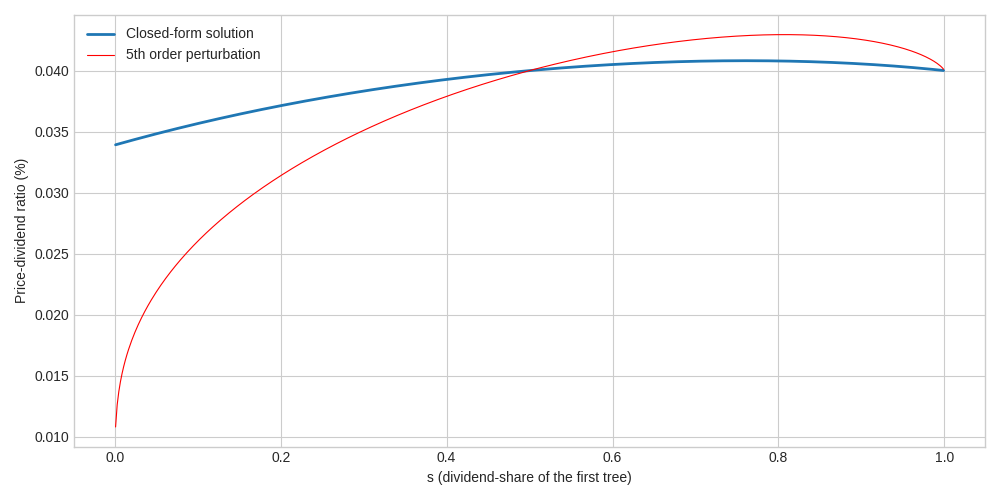
\includegraphics[width=0.8\textwidth]{../figures/poster.png}}}
      \centering
      \tiny
      \href{https://www.dropbox.com/s/5n0w1x44nk51iai/animation.gif?dl=0}{link}
    \end{figure}
    % \begin{figure}[H]
    %   \centering
    %       \frame{
    %     \movie{
\includegraphics[width=0.8\textwidth]{poster.png}}{animation.avi}}
    % \end{figure}
  \end{frame}
  
%   \begin{frame}{Animation}
%       \noindent\animategraphics[autoplay,loop,every=2,width=\linewidth]{25}{figures/animation.pdf}{1}{200}
%   \end{frame}

  \begin{frame}{HAM - Practical issues}
    \begin{wideitemize}
      \item Recursive formulation is not practical because of nested derivatives
          $$
            V_k = \frac{U_k + \mathbb{E}\left[\frac{dV}{dt}\right]_k}{\delta}
          $$
      \item Solution: project the value function using a basis (Neural Tangent Kernel) and do {\bf one high-order} Taylor expansion
      \item How implement high-order Taylor expansions?
      \begin{itemize}
        \item \href{https://openreview.net/pdf?id=SkxEF3FNPH}{Taylor-Mode Automatic Differentiation for Higher-Order Derivatives in JAX (2019)}
      \end{itemize}

    \end{wideitemize}
  \end{frame}
  
  \begin{frame}{HAM with Kernels}
    \begin{itemize}
      \item Impose:
        $$
          V(s) = V_0(s) + \epsilon \phi(s)^T \Theta_1 + \epsilon^2 \phi(s)^T\Theta_2 + \ldots
        $$
      \item The problem is still linear! Now in $\Theta$.
      \item Each term $\Theta_k$ can be solved with linear least squares
        \begin{itemize}
          \item $\Phi \Theta_k = target(\Theta_0, \Theta_1, ..., \Theta_{k-1}) $
          \item Because the same $\Phi$ shows up for every order, just need one SVD/Cholesky decomposition.
        \end{itemize}
      \item 5th order solution run time for the 2 Trees example: 5ms
    \end{itemize}
  \end{frame}


\begin{frame}{Next steps}
    \begin{wideitemize}
      \item Use this technique to solve our model\vspM
      \item Allows for quantitative results
    \end{wideitemize}
  \end{frame}

\begin{frame}[standout]
        Thanks!
\end{frame}

% \begin{transitionframe}
%   \begin{center}
%     { \Huge \textcolor{black}{Thanks!}}
%   \end{center}
% \end{transitionframe}

\begin{frame}{Second-order terms}\label{second_order}
    \hyperlink{first-order}{\beamerbutton{Back}}
\end{frame}

\end{document}
